\section{Data Link Layer}
\paragraph{Schicht 2: Sicherungsschicht}

\begin{definition}{Framing (Rahmenbildung-/erkennung)}
    \begin{itemize}
        \item Senderichtung: Einpacken der zu sendenen Nutzdaten in Datenrahmen (Frames)
        \item Empfangsrichtung: Erkennung und Auspacken der Datenblöcke aus empfangenen Frames
    \end{itemize}
\end{definition}

\begin{concept}{Asynchron}
    {\small Keine Daten → Nichts gesendet (Pause zwischen Frames)}
    \begin{itemize}
        \item Zu Beginn eines Frames wird ein Start-Bit gesendet
        \item Prüfbits am Ende eines Frames!
        \item Frame-Grenze gibt auch Byte-Grenze
    \end{itemize}
\end{concept}

\begin{concept}{Synchron}
    {\small ohne Unterbruch $\rightarrow$ kontinuierlicher Bitstrom auf Phy. Layer}
    \begin{itemize}
        \item Stehen keine Daten an, werden Flags gesendet (anstatt Pause)
        \item Frames werden durch ein Start-Flag und ein End-Flag begrenzt:
    \end{itemize}
    \begin{minipage}{0.6\linewidth}
        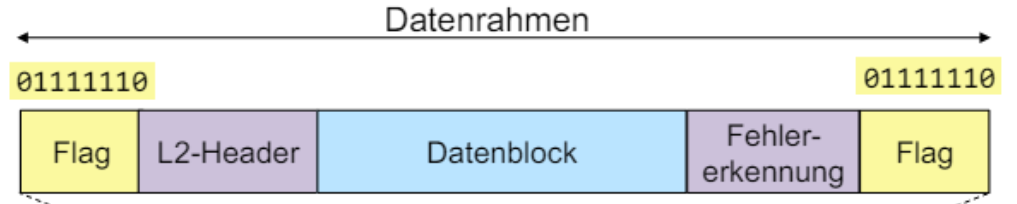
\includegraphics[width=1\linewidth]{images/flags_frames.png}
    \end{minipage}
    \begin{minipage}{0.39\linewidth}
        Maskierung von\\ Sonderzeichen (Flags)\\ nötig!
    \end{minipage}
\end{concept}

\begin{concept}{Bitstopfen} $\rightarrow$ um Bit-Muster zu garantieren 
    \begin{itemize}
        \item Sender fügt im Datenstrom nach 5 Einsen immer eine Null ein
        \item Empfänger wirft nach 5 Einsen immer ein Bit weg
        \item Somit gibt es (ausser bei Flags) nie die Bitfolge 01111110
    \end{itemize}
\end{concept}

\subsubsection{Framelänge und Fehlerwahrscheinlichkeit}

\begin{definition}{Fehlerwahrscheinlichkeit}
    \begin{itemize}
        \item BER (Bit Error Ratio) = 0.5 $\rightarrow$ jedes 2. Bit falsch
        \item FER (Frame Error Ratio): Fehlerhaft empfangene Frames
        \item RER (Residual Error Ratio): Unentdeckte fehlerhafte Frames
    \end{itemize}
\end{definition}

\begin{KR}{Frame-Fehlerwahrscheinlichkeit}

    Wahrscheinlichkeit dass Frame der Länge N min. 1 Bitfehler enthält:

    \vspace{0.5mm}

    $BER = p_e << 1 \longrightarrow (1 - p_e)^N \approx (1 - N \cdot p_e)$
    $$ \Rightarrow P_{Fehler, Frame} \approx N \cdot p_e (=FER)$$
\end{KR}

\begin{theorem}{Wahl der Framelänge} Overhead vs geringe Fehlerwahrscheinlichkeit
    \begin{itemize}
    \item Lange Frames:
    \begin{itemize}
        \item Höhere Nutzdatenrate ($\uparrow$ Netto-Bitrate, $\downarrow$ Overhead)
        \item $\Uparrow$ Fehlerwahrscheinlichkeit und Datenverlust pro Fehler 
        \item $\Uparrow$ Wahrscheinlichkeit eines unentdeckten Fehlers
    \end{itemize}
    \item Kurze Frames: Tiefere Nutzdatenrate, Zuverlässig
    \end{itemize}
\end{theorem}



\begin{formula}{Framelänge}
    Nettobitrate = Bruttobitrate $\cdot \frac{Nutzdaten}{Nutzdaten + Header}$
\end{formula}

\begin{formula}{Datenraten}  $F_R = \frac{B}{8\cdot(F_L + IFG)} \quad \quad \quad N = F_R \cdot P \cdot 8$ 
\end{formula}

\begin{remark}
    $F_R$ = Framerate, B = Bitrate, $F_L$ = Framelength, \\ IFG = Interframe Gap, N = Nutzbitrate, P = Payload
\end{remark}

\paragraph{Fehlererkennung und -korrektur}

\begin{concept}{Fehlererkennung} Redundanz $\rightarrow$ erhöht Hammingdistanz\\
    Zuverlässigkeit: abhängig von Framelänge/Verfahren
\end{concept}

\begin{remark}
    Standards IEEE 802 (LAN-Standards, zb Ethernet): 
    max. $5 \cdot 10^{-14}$ unentdeckte Fehler pro Frame-Byte,
    BER $p_e \leq 10^{-8}$ (1 Bitfehler pro 100 Mio. Bit)
    $\rightarrow$ CRC32 für Ethernet, mit Generatorpolynom (erkennt Fehler nur, korrigiert nicht)
\end{remark}

\begin{concept}{Fehlerkorrektur - Error Correction (EC)}
    \begin{itemize}
        \item Backward (BEC): erneutes Übertragen der Daten
        \item Forward (FEC): Rekonstruktion verfälschter Bits bei Empfänger
    \end{itemize}
\end{concept}

\begin{formula}{Hamming-Distanz} (h)
    \begin{itemize}
        \item Fehlererkennung: (h - 1) Fehler erkennbar
        \item Fehlerkorrektur: max. $\frac{h - 1}{2}$ Fehler korrigierbar
    \end{itemize}
\end{formula}

\begin{formula}{Einfache Parity}
    Prüfbit sichert ein Datenwort (typisch 1 Byte)\\
    Even Parity: Anzahl 1en inkl. Parity-Bit ist gerade (Odd analog)
\end{formula}

\begin{formula}{Längs- und Quer-Parity}\\
    3 Paritätsbits: 1 für jedes Byte, 1 für jedes Bit (Längs- und Quer-Parity), Gesamtparity

    \vspace{1mm}

    Korrigieren: 1 Bit-Fehler, Erkennen: 2 Bit-Fehler
\end{formula}


\subsubsection{Zugriffsmechanismen (Media Access)}

\paragraph{Gesteuerter Medium Zugriff}

\begin{definition}{Master-Slave Verfahren} Koordinierter Zugriff auf Medium
    \begin{itemize}
        \item Vorteil: Keine Konflikte, Master koordiniert Zugriff
        \item Nachteil: Ausfall des Masters (Single Point of Failure)
    \end{itemize}
\end{definition}

\begin{definition}{Token Verfahren} Sendeberechtigung in fixer Reihenfolge\\
    Knoten senden nur, wenn sie ein Token halten
    \begin{itemize}
        \item Vorteil:  Deterministisch (man weiss, wann man dran kommt)
        \item Nachteil: Aufwändiges Token Management (Startup, Token Verlust, etc.)
    \end{itemize}
\end{definition}

\begin{definition}{Zeitgesteuerter Zugriff} wie Taktfahrplan im Bahnnetz
    \begin{itemize}
        \item Vorteil: Optimierung möglich (nach Auslastung, Durchsatz, etc.)
        \item Nachteile: Planung und genaue Zeit in allen Knotepunkten erforderlich, Konflikte mit unplanbarem Verkehr
    \end{itemize}
\end{definition}

\paragraph{Random Medium Zugriff}

\begin{definition}{Carrier Sense Multiple Access} Vor Senden geteiltes Übertragungsmedium abhören ob frei (Carrier Sense), sonst bis Pause warten
    \begin{itemize}
        \item Vorteil: Alle Stationen gleichberechtigt (kein Master) \\ $\rightarrow$ jederzeit Zugriff auf Übertragungsmedium
        \item Nachteil: Kollisionen möglich (Collision Detection)
    \end{itemize}
\end{definition}

\begin{concept}{Kollisionsbehandlung - CSMA}
    \begin{itemize}
        \item CD (Collision Detection): Kollision: abbrechen, später nochmals
        \item CR (Collision Resolution): Hardware-unterstützte Arbitrierung
        \begin{itemize}
            \item Kollisionen werden erkannt und kontrolliert aufgelöst
        \end{itemize}
        \item CA (Collision Avoidance): Kollisionen vermeiden
        \begin{itemize}
            \item Request to Send / Clear to Send
        \end{itemize}
    \end{itemize}
\end{concept}

\begin{concept}{Flow-Control}\\
    Explizite Start-Stopp Signalisierung:
    \begin{itemize}
        \item Obere und untere Limite, stopp wenn oben, start wenn unten
    \end{itemize}
    Implizites Stop-and-Wait: Sender wartet auf ACK vor Senden
\end{concept}